%!TEX root = thesis.tex
\chapter{2-D Imaginary Time Evolving Block Decimation}
\label{chapter:2ditebd}

In this chapter we introduce some different ways to implement two-dimensional imaginary time-evolving block decimation and apply them in calculation of ground state of Heisenberg and transverse Ising model on two-dimensional square lattice. In section \ref{ite} and \ref{itebd}, we briefly review the idea of imaginary time evolution (iTEBD),[\ref{vidal}] and explain how to extend it to two-dimensional [\ref{X,zhon}]. Second, we briefly review another method to make 2D-iTEBD more stable[\ref{1.1}]. In the last section \ref{2dopt}, we record various particulars which are helpful optimizing algorithms.

\section{Imaginary Time Evolution}
\label{ite}
Theoretically, if having the imaginary time evolution operator $e^{-\tau H}$, we could project any random states to the ground state, as long as the wave-function can be written as,
\begin{align}
	\label{mapgroud}
	\Ket{\psi_0} = \frac{e^{\tau H} \Ket{\Psi}}{\parallel e^{\tau H} \Ket{\Psi}\parallel}
\end{align}
but according to the eq.\ref{mapgroud}, we may found that the number of coefficients in an origin evolution operator $e^{-\tau H}$ is proportional to $2^N \times 2^N$. On the other words, it is impossible to update entire system directly. In order to restricting the rapid dimensional growth, we apply \textit{Suzuki Trotter decomposition}[\ref{1.1}][\ref{1.1}] to approximate. The main idea of \textit{Suzuki Trotter} is decomposing the whole system to lots of units cell and using some smaller operations to update the wave-function.
\begin{align}
	\label{STd}
	e^{\delta A + B} = e^{\delta A}e^{\delta B} + O(\delta^2)
\end{align}
eq.\ref{STd} means the first-order Suzuki Trotter  decomposition, and A and B are non-commutative with each other.

Now that the dimension of the evolution operator is reduced to a n-site operator and in chapter \ref{chapter:properties}, we have shown that a many-body system can map to a MPS or PEPS structure, so we can draw the process of updating a ground state like Fig.\ref{fig312},

\begin{figure}[ht]
	\centering
	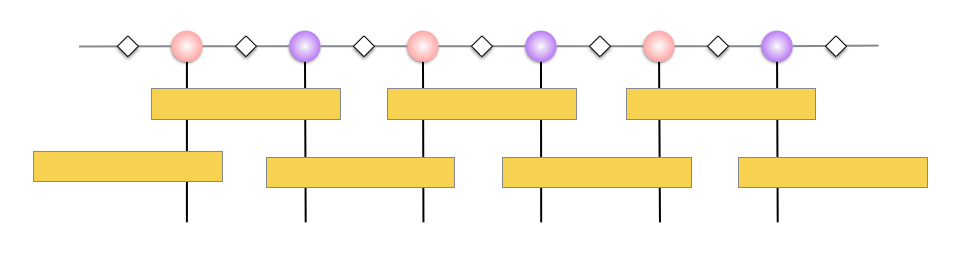
\includegraphics[width=0.75\textwidth]{figures/fig312.png}
	\caption[The picture of the main idea of itebd.]{The red and blue tensor denotes on \textit{odd} and \textit{even} sites. The yellow one are time evolution operators $e^{-\tau H_{k,k+1}}$, $e^{-\tau H_{k+1,k}}$}
	\label{fig312}
\end{figure}

On the other work, contract the tensors in Fig.\ref{fig312} repeatedly until the ground state energy to the minimum. The remained tensor is considered as the ground state of the system. So the next question: How can we contract them and preserve the structure like Fig{\ref{fig311}}? This answer is iTEBD.

\begin{figure}[ht]
	\centering
	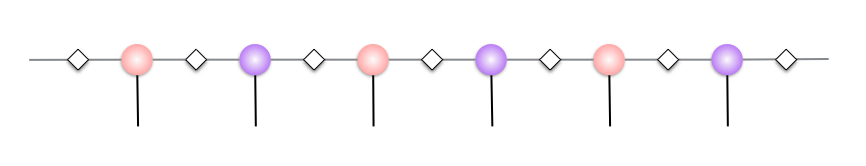
\includegraphics[width=0.75\textwidth]{figures/fig311.png}
	\caption[The picture of matrix product states]{The simple form of a matrix product state.}
	\label{fig311}
\end{figure}

\section{Simple Infinite Imaginary-Time Evolving Block Decimation for 2-D system}
In this section, we apply the TN diagrams to introduce the methods of implementation of algorithm. If you are interested in the mathematical formula of them, please read the references \citep{vidal_efficient_2004} [\ref{dd}][\ref{eaef}], witch include more details of theoretical discussion.

\label{itebd}
\subsection{Simple Description of iTEBD for 1-D system}

The algorithm start from 2 random states and 2 random diagonal matrices which are considered as entanglement between particles. In the TN diagrams, Fig.\ref{fig313}, the states and entanglement between neighbor sites are represented by the nodes and bonds with different colors.

\label{1ditebd}
\begin{figure}[ht]
	\centering
	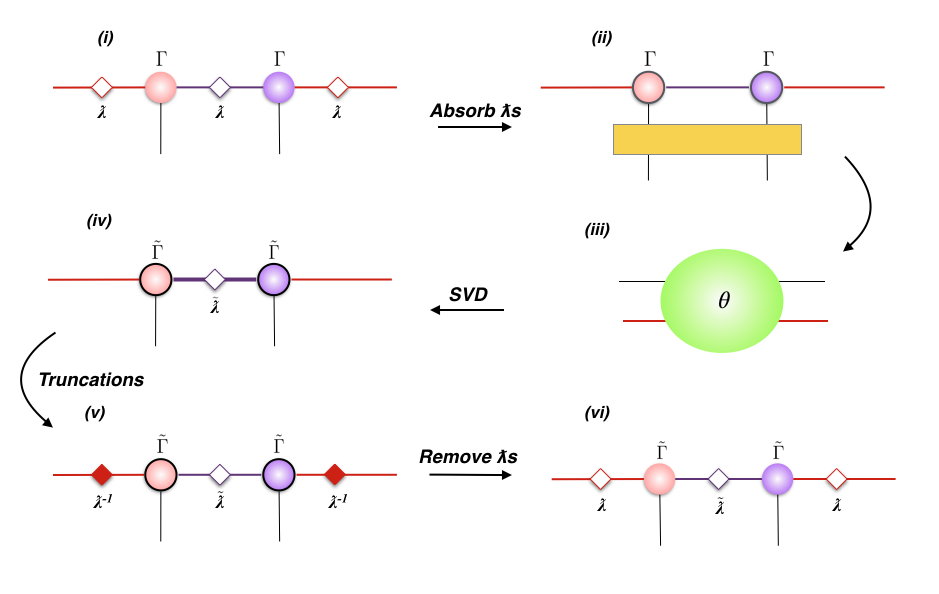
\includegraphics[width=0.90\textwidth]{figures/fig313.png}
	\caption[The tensor network diagrams for the 1-D iTEBD]{ (i)Absorb all $\lambda$ to $\Gamma$. (ii) Contract an evolution operator $e^{-\delta H}$ for evolving the system. (iii) Decompose the tensor $\theta$ by SVD. (iv) Truncate and Update the states and $\lambda$ on the green bond.(v) Remove $
		\lambda$ for obtaining the states. (iv) After updating the states and $\lambda$ on the purple bond, apply the way to update the red bond and repeat all the steps until the ground state convergence.}
	\label{fig313}
\end{figure}

The processes shown in Fig.\ref{fig313} is a standard strategy for implementation of iTEBD and also called \textit{Simple Update}. 

In one dimensional system, the performance of Simple Update is pretty well, because 1-D systems obey the canonical form and have less influences of environment. However, in 2-D systems, due to the area law, we need consider the environment more restrictively when measuring the local observable. Moreover, the computational consumption is another serious problem, owing to the growth of a state's dimension which is proportional to $dD^4$.

In order to solving that obstacles, optimizations of 2-D algorithms  became an important part in condense matter physics. This chapter we focus on obtaining good enough projected entangled pair states from 2-D iTEBD and the strategies of improving measurement would be shown in following chapters.

\subsection{Description and Pseudocode of iTEBD for 2-D system}
\label{2ditebd}

Now that we stated to extend it to a two dimensional system. In chapter.\ref{chapter:properties}, we have known that a two dimensional many-body system is able to be represented by PEPS. Due to impossibly drawing an network of infinite sites, the structure of infinite PEPS (iPEPS) is decided by the geometry of the lattice and the unit cell we chosen. In usual, the size of unit cell depend on the n-site evolution operator. For instance, if the target is updating iPEPS of a square lattice with 2-site operator, the tensor diagram would be drawn as Fig.\ref{fig314}.

\begin{figure}[ht]
	\centering
	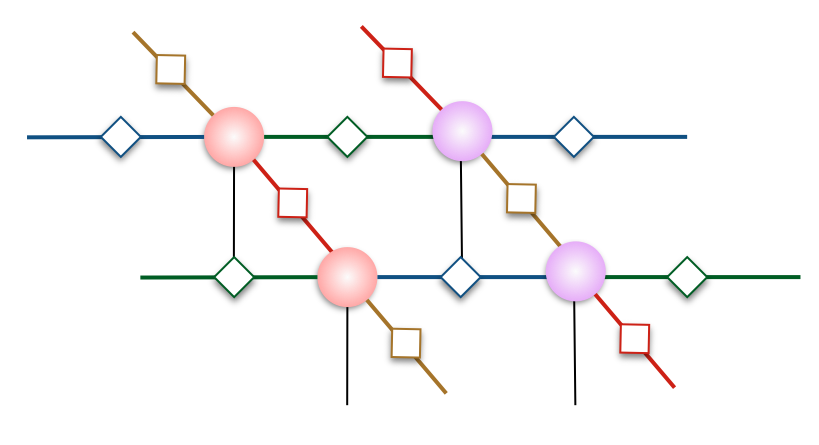
\includegraphics[width=0.6\textwidth]{figures/fig314.png}
	\caption[The tensor diagrams of 2-D lattice]{Four sites unit cell in iPEPS.}
	\label{fig314}
\end{figure}

After setting the form of iPEPS, we start to deal the question of updating states. The most intuitive scheme is to apply the scheme of \textit{Simple Update} which is shown in Fig.\ref{fig315}. The steps are similar to the iTEBD on 1-D systems. However, there are some differences. Firstly, the projected entangled pair states is a rank-5 tensor. Secondly, there are more entangled should be considered, due to increased neighbor sites.

More theoretical descriptions are written in [\ref{}][\ref{}]. Here, we explain the methods with TNs and some simple pseudocodes. The basic idea of \textit{2-D iTEBD} is to update the states from four directions by \textit{Simple Update}. The example starting from updating the green bond is shown in Fig.\ref{fig315} and Fig.\ref{fig316},

\begin{figure}[ht]
	\centering
	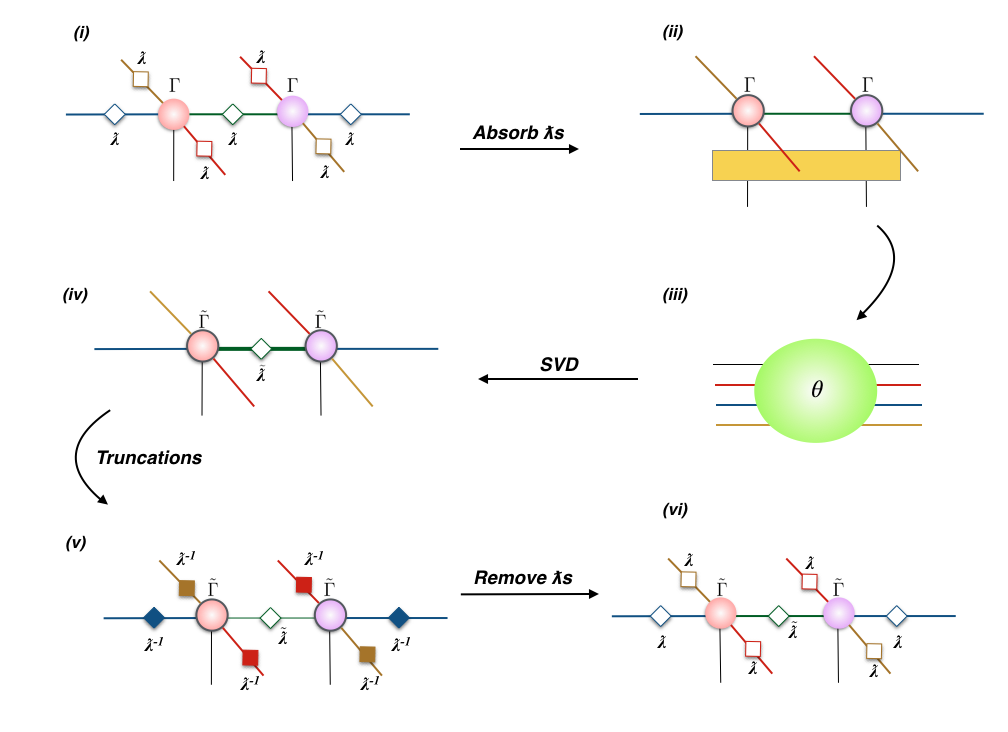
\includegraphics[width=1.00\textwidth]{figures/fig315.png}
	\caption[The tensor network diagrams of updating the green bond in iPEPS with 2D-iTEBD]{Absorb all $\lambda$ to $\Gamma$. (ii) Contract an evolution operator $e^{-\delta H}$ for evolving the system. (iii) Decompose the tensor $\theta$ by SVD. (iv) Truncate and Update the states and $\lambda$ on the green bond.(v) Remove $\lambda$ for obtaining the states. (iv) Obtain a original form of iPEPS. Repeat all the step to update the other bonds until the ground state energy convergence}
	\label{fig315}
\end{figure}

It's the same as one dimensional case, The first step is to absorb all $\lambda$ around the sites. The tensor with gray bold means the state have absorbed all entanglements. Secondly, contract the gate, $e^{-\delta H}$, for getting the tensor $\theta$. Thirdly, apply singular value decomposition to update states and the entanglement on the green bond. After decomposing $\theta$, we found that the dimension of the green bond increase to $dD^4$. Therefor, truncation plays a significant roles for keeping the dimension in the algorithm. In the end of the updating processes, multiply pseudo inverse of all $\lambda$ to the tensors for reducing to original form. 

	\begin{figure}[ht]
	\centering
	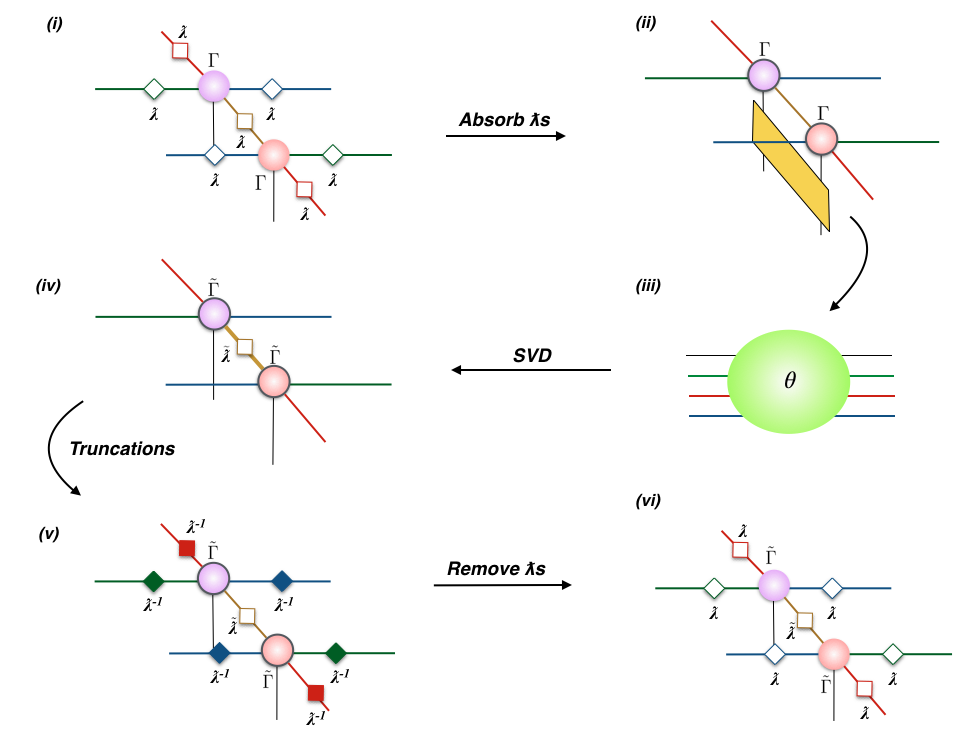
\includegraphics[width=1.00\textwidth]{figures/fig316.png}
	\caption[The tensor network diagrams of updating the yellow bond in iPEPS with 2D-iTEBD]{Update the yellow bond and the steps are similar to Fig.\ref{fig315}}
	\label{fig316}
	\end{figure}

	For easily to imagine how to updating the others directions. The updating steps of yellow bond are shown In Fig.\ref{fig316}.

%\begin{algorithm}
%	\caption{My algorithm}\label{euclid}
%	\begin{algorithmic}[1]
%		\Procedure{MyProcedure}{}
%		\State $\textit{stringlen} \gets \text{length of }\textit{string}$
%		\State $i \gets \textit{patlen}$
%		\BState \emph{top}:
%		\If {$i > \textit{stringlen}$} \Return false
%		\EndIf
%		\State $j \gets \textit{patlen}$
%		\BState \emph{loop}:
%		\If {$\textit{string}(i) = \textit{path}(j)$}
%		\State $j \gets j-1$.
%		\State $i \gets i-1$.
%		\State \textbf{goto} \emph{loop}.
%		\State \textbf{close};
%		\EndIf
%		\State $i \gets i+\max(\textit{delta}_1(\textit{string}(i)),\textit{delta}_2(j))$.
%		\State \textbf{goto} \emph{top}.
%		\EndProcedure
%	\end{algorithmic}
%\end{algorithm}


\section{Ameliorate two-dimensional iTEBD}
\label{2dhastin}

This method which make the algorithm more stable was published by \textit{M. B. Hastings}. Although \textit{Simple Update} shown in section.\ref{2ditebd} can obtain pretty good states, it's not stable and efficient enough. The reason is that too many multiplications of pseudo inverse $\lambda$ at the step Fig.\ref{fig315}(v). In numerical methods, it's hard to deal the problem of dividing the value which is equal or approach to zero. On the other words, the more inverse operations, the more the probability of bring about divergence or destroying algorithms.

For reducing the risk of breaking algorithms. Firstly, declare the states $\Gamma$ which include two entanglements among them. For instance, In Fig.\ref{fig317}(i), the red tensor is considered as multiplication of $A$ and the $\lambda$ on the yellow. The purple one is multiplication of $B$ and remained $\lambda$. Secondly, in Fig.\ref{fig317}(ii), because the entanglements on red and blue bonds are included in tensor $B$, we just need absorb the yellow one and contract the evolution operation for obtaining tensor $C$. Thirdly, we contract the red and blue $\lambda$ to the red and blue bonds which belong to the original tensor $A$ in tensor $C$ for getting $\theta$. Fourthly, getting the $\tilde{B}$ from decomposing and truncating $\theta$. Owing to avoid multiplying inverse matrices, we get $\tilde{A}$ by contracting tensor $C$ and $\tilde{B}$ and multiply an inverse $\lambda$ of yellow bond for removing the entanglement and reducing to original form.

	\begin{figure}[ht]
	\centering
	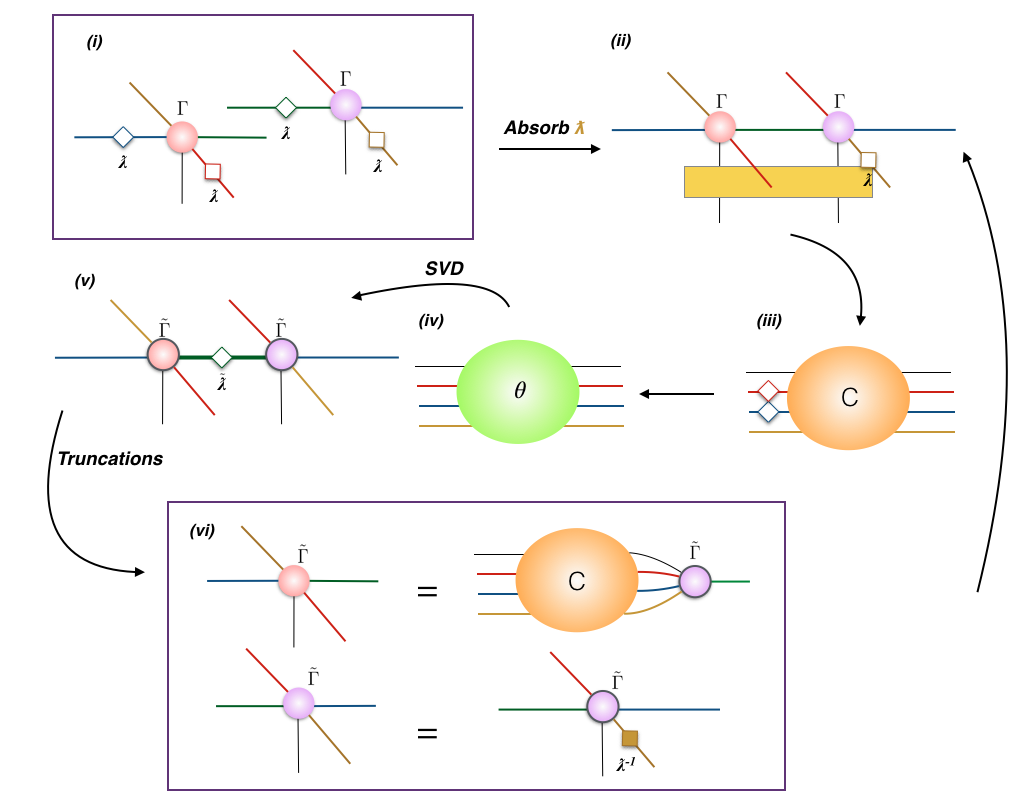
\includegraphics[width=1.00\textwidth]{figures/fig317.png}
	\caption[The tensor network diagrams for the 2-D iTEBD with QR decomposition]{The tensor network diagrams for the ameliorated 2-D iTEBD.}
	\label{fig317}
	\end{figure}

	Finally, repeat all the processes shown in Fig.\ref{fig317} to update different bonds until the convergence of the ground state energy.

\section{Optimizations}
\label{2dopt}

\subsection{Initialization}
\label{2doptInit}
Intuitively, the initialization of states should not affect the result. However, it's a serious misunderstanding. Actually, stating from a awful initial sates may break the algorithms or hardly converge.

From the viewpoint of physics, translational invariance is one of essential properties in many-body system, So we can assume that the group state on two sites should be similar. For instance, if the TN diagram of the states is shown as Fig \ref{fig321}(i), Fig \ref{fig321}(ii) might be the better way to initialize the states.

\begin{figure}[ht]
	\centering
	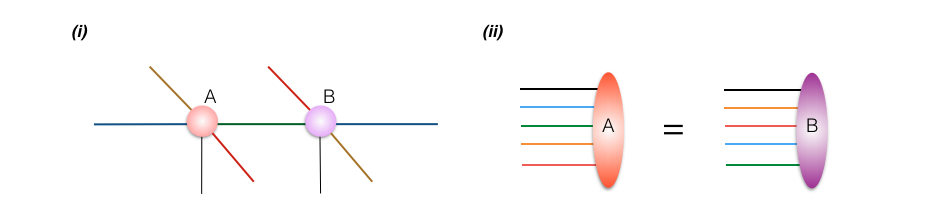
\includegraphics[width=1.00\textwidth]{figures/fig321.png}
	\caption[The diagrams of initializing projected entangled pair states]{(i) The structure of PEPS, (ii) The initialization of states}
	\label{fig321}
\end{figure}

\subsection{Truncattion Error}

\subsection{QR decomposition}

Though the strategy described in previous sections improve the stability, it's not efficient enough. The reason why is that the dimension of tensor $\theta$, in Fig.\ref{fig315}(iii) and Fig.\ref{fig317}(iii), is proportional to $d^2D^6$. In addition to that, the time complexity of singular value decomposition is proportional to $O(NM^2)$. In conclusion, the steps, in Fig.\ref{fig315}(iii) and Fig.\ref{fig317}(iii), are expensive, it is necessary to reduce the dimension of tensor $\theta$. 
\label{2doptQR} \begin{figure}[H] \centering 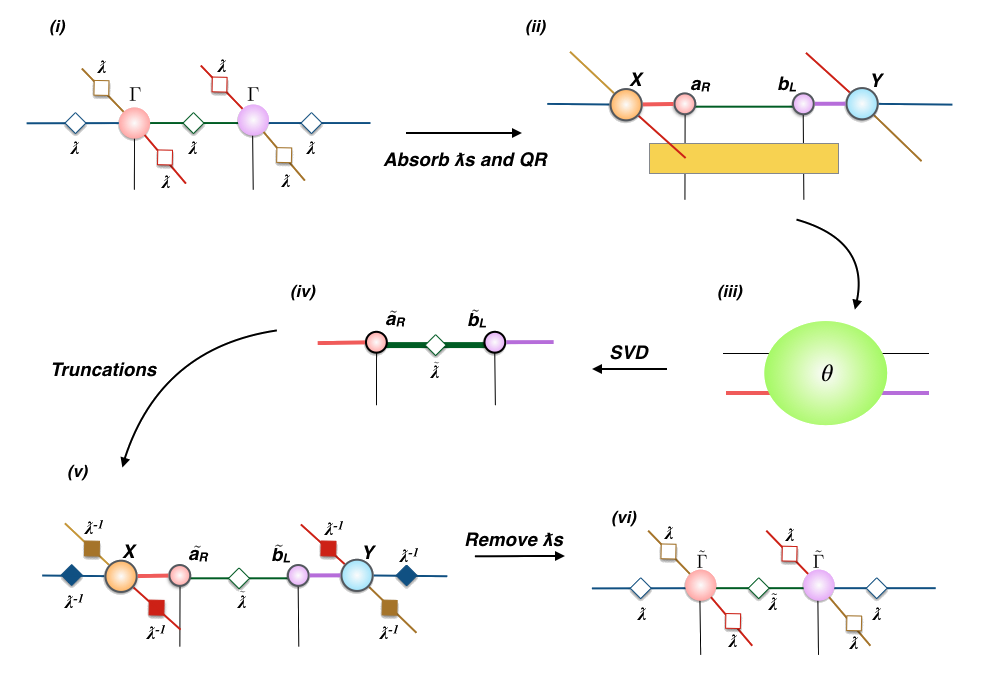
\includegraphics[width=0.80\textwidth]{figures/fig318.png} \caption[The tensor network diagrams for the ameliorated 2-D iTEBD with QR decompositiont]{The tensor network diagrams for the ameliorated 2-D iTEBD.} \label{fig318} \end{figure} To achieve the goal, the projected pair state must be decomposed by QR decomposition. The processes making \textit{Simple Update} more efficient is illustrated in Fig \ref{fig318}.  Most of the steps shown in Fig \ref{fig318} are like in Fig \ref{fig315}. The only difference is that after absorbing all the $\lambda$, we decompose the state to an orthogonal matrix and an upper triangular matrix by QR. For instance, in Fig \ref{fig318} (ii), the state $A$ is decomposed to an orthogonal matrix X and upper triangular matrix $a_R$. Due to the columns of $X$ are orthonormal, $XX^{\dagger}$ is equal to $I$. In the other word, the tensor $X$ can be ignored and we just need consider the tensor $a_R$ by QR. Similarity, the state $B$ can be decomposed to a lower triangular $b_L$ and an orthogonal matrix $Y$ by LQ which is equivalence to operate QR decomposition after transpose the matrix. Next, (iii) we can obtain the tensor $\theta$ whose dimension is $d^2D$ from $a_R$, $b_L$ and an evolution operator.

\begin{figure}[ht]
	\centering
	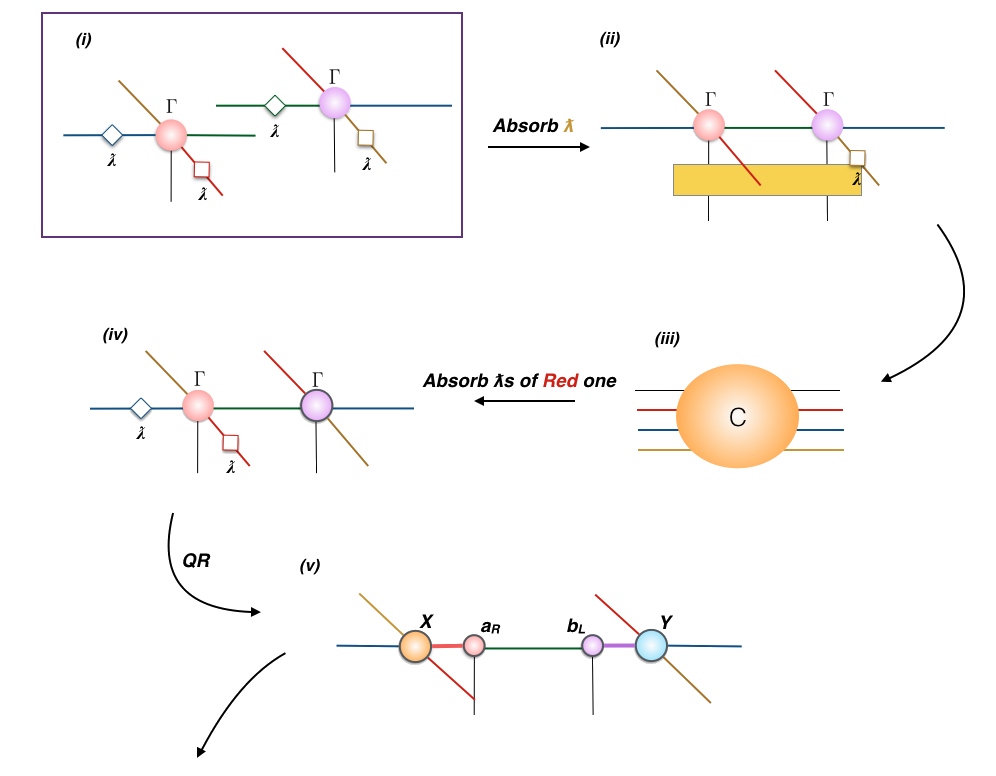
\includegraphics[width=0.90\textwidth]{figures/fig319.png}
	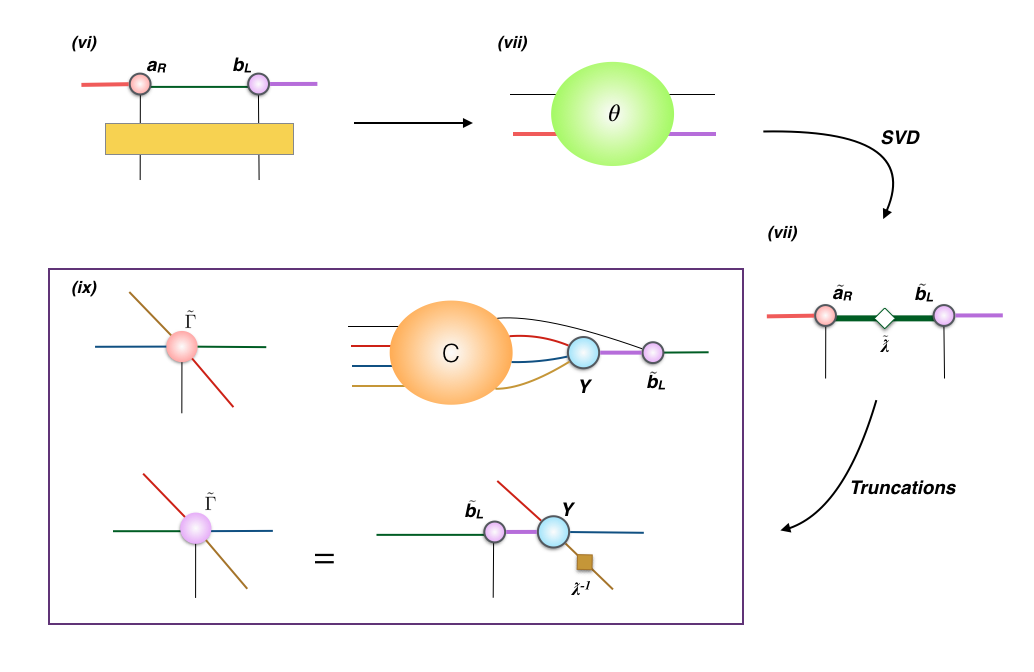
\includegraphics[width=0.90\textwidth]{figures/fig320.png}
	\caption[The tensor network diagrams for the ameliorated 2-D iTEBD with QR decompositiont]{The tensor network diagrams for the ameliorated 2-D iTEBD.}
	\label{fig319}
\end{figure}

The strategy to accelerate \textit{Ameliorate Simple Update} is shown in the Fig \ref{fig319} and its main idea is also to reduce the dimension of $\theta$.

\section{Comparison}

So far, we have benchmarked the improved iTEBD. 

\label{Comparison}
\subsection{Different Initializations}

\begin{figure}[ht]
	\centering
	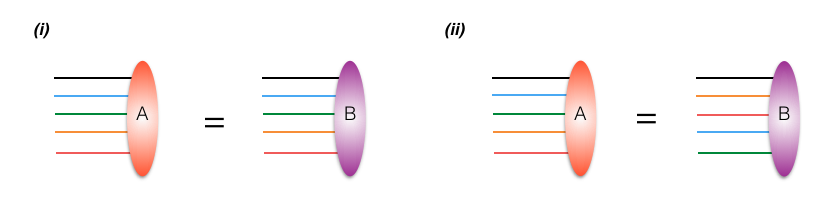
\includegraphics[width=1.00\textwidth]{figures/fig322.png}
	\caption[Different methods to initialize the states]{(i) Type 1, (ii) Type 2}
	\label{fig322}
\end{figure}

See Fig \ref{fig323}, the both cases are 

\begin{figure}[ht]
	\centering
	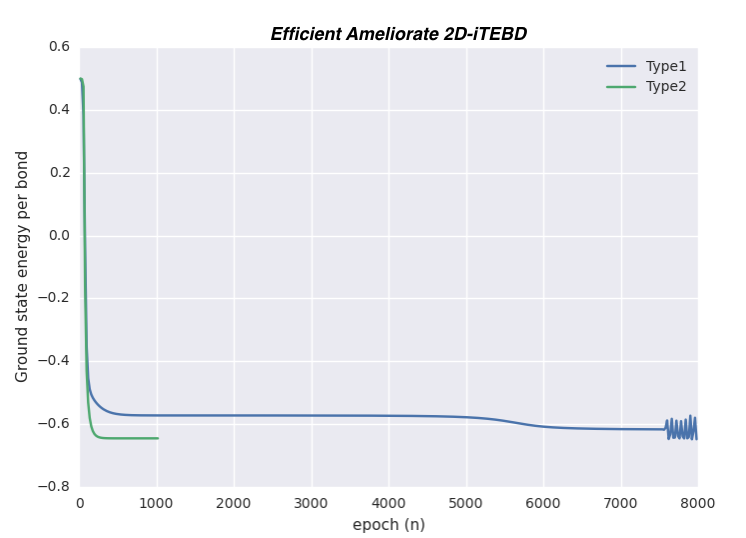
\includegraphics[width=0.75\textwidth]{figures/fig323.png}
	\caption[Comparison the results of Heisenberg model on square lattice which are obtaining from different initial states.]{The Blue line represents updating tensors from the initial state shown in Fig \ref{fig322} (i) and the green one represents updating from Fig \ref{fig322} (ii)}
	\label{fig323}
\end{figure}

\begin{figure}[ht]
	\centering
	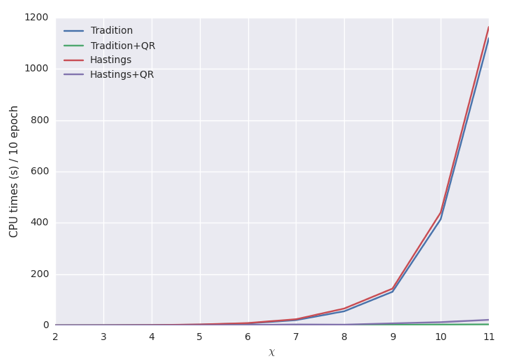
\includegraphics[width=0.75\textwidth]{figures/fig324.png}
	\caption[tmp]{}
	\label{fig324}
\end{figure}

\begin{figure}[ht]
	\centering
	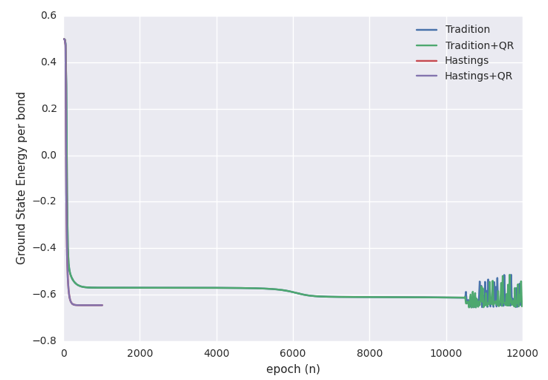
\includegraphics[width=0.75\textwidth]{figures/fig325.png}
	\caption[tmp]{}
	\label{fig325}
\end{figure}

\begin{figure}[ht]
	\centering
	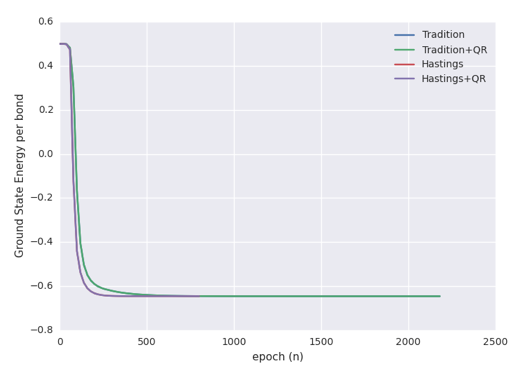
\includegraphics[width=0.75\textwidth]{figures/fig326.png}
	\caption[tmp]{}
	\label{fig326}
\end{figure}

\begin{figure}[ht]
	\centering
	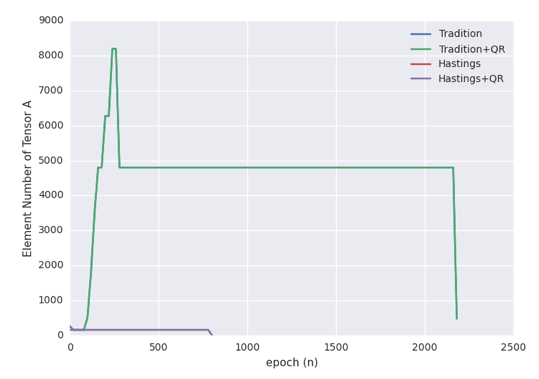
\includegraphics[width=0.75\textwidth]{figures/fig327.png}
	\caption[tmp]{}
	\label{fig327}
\end{figure}
